\chapter{Related Work
    \pgsize{15 p.}
}
\label{chap:relatedwork}

\begin{figure}
    \centering
    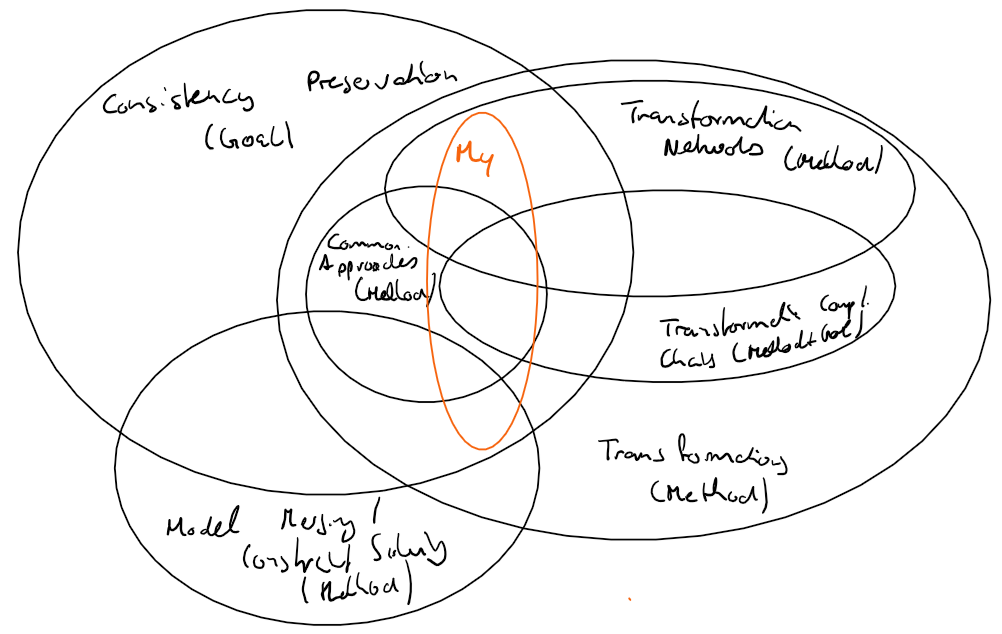
\includegraphics[width=\textwidth]{figures/epilogue/relatedwork/research_areas.png}
    \caption[Overlaps of related research areas]{Sketch of different research areas related to the work of this thesis, the overlaps, and the embedding of this thesis in those areas.}
    \label{fig:relatedwork:areas}
\end{figure}

\section{Consistency Preservation}
Roundtrip Engineering
MPM
Multi-View survey ~\cite{cicchetti2019multiview-SoSym}

\section{Transformation Networks}

\section{Multidirectional Transformations}

\section{Commonalities Approaches}
OSM

Bezug zu \enquote{Weaves} in \cite{kolovos2008a}: Additional model for relating models. Originally focused on trace models, but auxiliary models such as commonalities can also be considered as such

\section{Transformation Chains and Composition}

\section{Model Merging and Constraint Solving}



\todo{Sequentialisierung vs. Merging diskutieren -> Bisimulation}

\begin{copiedFrom}{DocSym}

\section*{From DocSym Overview}
% MULTI-MODEL CONSISTENCY AS A WHOLE
\emph{Model consistency preservation}, also referred to as %\emph{model synchronization} or 
\emph{model repair}, is an active field of current research. 
Nevertheless, most approaches are restricted to consistency between pairs of models~\cite{stevens2020BidirectionalTransformationLarge-SoSym}.
The kinds of dependencies between multiple models and types of inconsistencies were discussed by \textcite{kolovos2008a}. 
A summary and classification of model consistency approaches, also regarding their multi-model support, was presented by \textcite{macedo2015a}.

% BINARY TRANSFORMATIONS LANGUAGES AND EXTENSIONS
As stated by \textcite{stevens2020BidirectionalTransformationLarge-SoSym}, it is reasonable to target multi-model consistency by combining binary transformations.
%Multi-model consistency can also be achieved by combining mechanisms for consistency preservation between pairs of models. 
Especially incremental model transformation languages %, which update models after changes to restore consistency, 
can be applied by executing the transformations transitively.
They were surveyed by \textcite{etzlstorfer2013SurveyIncrementalTransformation-ME}, including the \gls{ATL}~\cite{jouault2006a,xiong2007a}, VIATRA~\cite{bergmann2015viatra} and \glspl{TGG}~\cite{anjorin2014b,anjorin2014c}. 
For \glspl{TGG}, initial concepts for supporting multiple models were proposed~\cite{trollmann2015TransformationTGGtoMultiModel-ICMT,trollmann2016SynchronizationTGGtoMultiModel-ICMT}. 
Another transformation-based tool is \emph{Echo}~\cite{macedo2013b}. 
It is based on \emph{Alloy}~\cite{macedo2013a}, which uses \mbox{QVT-R}~\cite{qvt} and model finding to repair inconsistencies. 
For \mbox{QVT-R}, challenges and steps towards supporting transformations between multiple model were discussed~\cite{macedo2014FrameworkMultiDirectional-BX}.
\citeauthor{kramer2017a} proposed an approach combining a language for declarative mappings between metamodels with a fallback language for imperative consistency repair~\cite{kramer2017a, klare2016b}, developed in the context of the \vitruv framework~\cite{kramer2015a}. %, on which our approach will be based as well.
Except for the explicitly mentioned works, those approaches do not explicitly deal with challenges introduced by combining binary transformations.
%All transformation-based approaches specify consistency relations implicitly in their transformations, whereas our approach makes the commonalities of metamodels explicit. Furthermore, combining pairwise specifications has several drawback, which we will discuss in the following section.
Another topic regarding transformations is \emph{uncertainty}. Not all decision can be made automatically, e.g., whether a created Java class shall represent an \gls{ADL} component or not. To handle this, different solutions can be calculated~\cite{eramo2015uncertainty-SLE} or the developer can be asked for his intent~\cite{langhammer2014a}.

% COMPOSITION APPROACHES
Approaches regarding the combination of binary transformations are rather focused on composing transformations between the same two metamodels~\cite{wagelaar2008a, wagelaar2010a, wagelaar2011a}.
Additionally, those approaches do usually not consider transformations as black boxes, but provide intrusive composition operators that require adaptions of the composed transformations~\cite{cuadrado2008a}.
Some approaches also deal with processes for %transformation
composition %, especially the specification of composition, 
and simply assume interoperability~\cite{oldevik2005a}.

% COMMON CONCEPT REFACTORING
An approach specific for expressing and preserving consistency between different \glspl{ADL} is \dually~\cite{malavolta2010ADLInteroperability-TSE,eramo2012Dually-SoSym}. 
It requires the specification of relations between concrete \glspl{ADL} to a central, predefined \gls{ADL} metamodel.
\dually is based on a generic model consistency approach, which uses \gls{ASP}~\cite{cicchetti2006a,eramo2008a} based on logical programming techniques. %to validate consistency and calculate possible repair operations. 
%It is comparable to our approach using \acp{CMM}, but in contrast, it is specific for \acp{ADL} whereas our approach allows to integrate arbitrary metamodels. %, logical programming.
Such an approach of adding additional metamodels to represent consistency relations is also shortly discussed in \cite{stevens2020BidirectionalTransformationLarge-SoSym}. %, but with focus on definability of multiary relations instead of the optimization regarding certain challenges. % as we do.

There has also been research on design patterns for transformations~\cite{iacob2008a, lano2014a}.
They have been surveyed by \textcite{lano2018a}, but mainly unify how specific kinds of consistency relations can be expressed in transformation languages and not on achieving non-intrusive transformation interoperability.
%In contrast, the patterns we develop focus on non-intrusive interoperability of transformations.

% THE SUM APPROACH
%An approach that completely avoids consistency preservation is the \ac{OSM} approach~\cite{atkinson2010a}, which uses a \ac{SUM} to describe a complete software system.
%The metamodel of the \ac{SUM} has to be defined additionally and redundancy free, which requires high effort and disallows reuse of existing tooling but results in an inherently consistent \ac{SUM}.
%\ac{OSM} is comparable to a hybrid approach~\cite{cicchetti2011a}, which proposes the usage of a single metamodel from which views can be created on demand.

% \dually~\cite{malavolta2010ADLInteroperability-TSE}:
% \begin{itemize}
%     \item Approach for interoperability of different \acp{ADL} (even more than two) and tools
%     \item Specify relations of concrete \acp{ADL} to central, predefined \acp{ADL} metamodel
%     \item Central metamodel can be extended to avoid information loss
%     \item Central metamodel can be seen as VOMM for \acp{ADL}, thus, in contrast to our approach, it is predefined and thus context-specific, whereas our approach can be used to define that central \ac{ADL} metamodel, but others as well
%     \item Approach was extended by \textcite{eramo2012Dually-SoSym} with an approach based on \ac{ASP} for propagating changes across different \acp{ADL} to achieve consistency~\cite{cicchetti2006a,eramo2008a}. The \ac{ASP} approach requires the specification of models and correspondences between them as axioms and rules known from logical programming. With their evaluation, consistency can be validated and potential modifications for restoring consistency can be calculated
% \end{itemize}

% \ac{OSM}~\cite{atkinson2010a}
% \begin{itemize}
%     \item Idea of having a \ac{SUM}, which describes every aspect of a software system without redundancies and dependencies, thus having no inconsistencies
%     \item Is based on a \ac{SUMM}, which has to represent everything that has to be modeled
%     \item In a way, this is a multi-model consistency approach, as without the approach several models with inconsistencies would exist, while this approach integrates them into one model that is consistent by design
%     \item Especially existing metamodels have to be integrated into that \ac{SUMM}, requiring effort, loosing tooling for the existing metamodel and having the requirement of modeling everything dependency-free
%     \item In contrast to our approach, no consistency preservation is necessary, but high effort for creating the \ac{SUMM} is necessary (if even possibly without having redundancies or dependencies)
% \end{itemize}

% \begin{itemize}
%     \item The approach is also comparable to the hybrid approach presented by \textcite{cicchetti2011a}. They propose the usage of a single \modelinglanguage from which view can be created on demand and which are kept consistent by model differencing. The approach assumes that no concurrent modifications are performed.
% \end{itemize}

% Topic: Multi-model consistency checking

% \todo{Den folgenden Approach vielleicht weglassen, vor allem wenn es zu viele Referenzen sind}
% \begin{itemize}
%     \item \textcite{szabo2013a} propose an approach for defining correspondences between multiple \modelinglanguages and the possibility to assign actions to them that are performed after modifications of the systems for checking consistency. 
% \end{itemize}


% Topic: Bi-model consistency preservation
% \begin{itemize}
%     \item A commons approach for keeping two models consistency is the application of incremental model transformation languages. Incremental transformation languages were surveyed by \textcite{etzlstorfer2013SurveyIncrementalTransformation-ME}, including the \ac{ATL}~\cite{jouault2006a,xiong2007a}, VIATRA~\cite{bergmann2015viatra}, \acp{TGG}~\cite{anjorin2014b,anjorin2014c}. \citeauthor{trollmann2015TransformationTGGtoMultiModel-ICMT} proposed initial concepts for the extension of \acp{TGG} to support multiple models~\cite{trollmann2015TransformationTGGtoMultiModel-ICMT,trollmann2016SynchronizationTGGtoMultiModel-ICMT}. Nevertheless, \acp{TGG} still require the specification of transformations between models rather than the explicit specification of VOMMs as we propose.
%     \item A transformation-based tool presented by \citeauthor{macedo2013b} is \emph{Echo}~\cite{macedo2013b}. It is based on \emph{Alloy}, which uses QVT-R~\cite{OMG2016a} for model checking and model finding to repair inconsistencies~\cite{macedo2013a}. While most implementations of the QVT-R standard focus on supporting bidirectional transformations, \textcite{macedo2014FrameworkMultiDirectional-BX} also discussed challenges and steps towards the support of multidirectional transformations between multiple models.
%     \item A change-driven approach combining a language for declarative mappings between metamodels with a fallback language for imperative consistency repair routines was proposed by \textcite{kramer2017a}. It was developed in the context of the Vitruvius framework~\cite{kramer2015a} on which this approach will be based as well.
% \end{itemize}

\end{copiedFrom} % DocSym


\begin{copiedFrom}{ICMT}

\section*{From Interoperability Case Study}

%Model consistency preservation is a research topic of current interest. 
\textcite{macedo2017ModelRepairClassification-TSE} provide a classification of consistency preservation approaches also considering support for multi-model scenarios. %and especially compares whether approaches consider multi-model scenarios.
In the following, we compare our work to research areas related to preserving consistency between multiple model types.
%Our work focuses on approaches that preserve consistency rather than only checking them.
%We will therefore compare our approach to related research areas.

\subsection*{Networks of Bidirectional Transformations} 
Networks of bidirectional transformations are the focus of our research.
%We focus on networks of %binary and especially 
%bidirectional transformations. 
\textcite{stevens2020BidirectionalTransformationLarge-SoSym} investigates the ability to split global into binary constraints.
She gives arguments to stick to networks of bidirectional transformation rather than using multidirectional transformations. % and considers how n-ary relations can be split into sets of binary relations.
Important for such networks is the transformation execution order. 
While we aim to allow arbitrary execution orders, other approaches focus on finding or defining appropriate orders~\cite{stevens2020BuildingFromMegamodels-SoSym}.
%\todoHeiko{Add Correct-by-construction here \cite{lano2014a}}

% \begin{itemize}
%     \item Basic investigation by \cite{stevens2020BidirectionalTransformationLarge-SoSym}: Ability to separate global constraints into bidirectional transformation, argumentation for sticking to bx networks rather than multidirectional transformations
%     \item Orientation model to derive appropriate set of transformations to be executed after a specific change ~\cite{stevens2020BuildingFromMegamodels-SoSym}
%     \item Patterns for correct-by-construction synthesis (very related, take deeper look!)~\cite{lano2014a}
% \end{itemize}

\subsection*{Multidirectional Transformations}
Multidirectional transformations 
are an alternative to networks of bidirectional transformations.
Although they benefit from being less prone to interoperability issues, they do not allow for modular definitions of consistency specifications.
The QVT-R standard~\cite{qvt} considers multidirectional transformations, but \textcite{macedo2014FrameworkMultiDirectional-BX} reveal several limitations of its applicability.
An extension of \glspl{TGG} to multiple models~\cite{trollmann2015TransformationTGGtoMultiModel-ICMT, trollmann2016SynchronizationTGGtoMultiModel-ICMT} focuses on the specification of multidirectional rules but not on potential conceptual and operational issues that we investigated.
 %on multidirectional transformations 
Commonalities metamodels offer a different approach to reduce the number of transformations and potential issues.
\textcite{gleitze2017a} proposes a generic idea for them, whereas DUALLy~\cite{malavolta2010ADLInteroperability-TSE, eramo2012Dually-SoSym} uses a domain-specific commonalities metamodel for architecture description languages.
\textcite{stunkel2018MultimodelCorrespondence-ICPS} and \textcite{diskin2018MultiModelSynchronization-FASE} discuss such commonalities metamodels from a theoretical viewpoint.
Several topics of multidirectional transformations, especially the usage of networks of bidirectional transformations and the interaction of several bidirectional transformations, were discussed in a Dagstuhl seminar~\cite{cleve2019dagstuhl}.
The focus in related working groups was the investigation of scenarios, in which networks of bidirectional transformations do not suffice and thus checked our assumption in \autoref{chap:correctness:notions_consistency:monolithic_modular}.

% \begin{itemize}
%     \item Limitations of QVT-R for multidirectional transformations~\cite{macedo2014FrameworkMultiDirectional-BX}
%     \item Extending TGGs to multiple models, focused on specification of multidirectional rules with TGGs but not on conceptual and operational issues that may occur~\cite{trollmann2015TransformationTGGtoMultiModel-ICMT, trollmann2016SynchronizationTGGtoMultiModel-ICMT}
%     \item Specify commonalities metamodels to reduce of number of transformations~\cite{gleitze2017a}
%     \item Domain-specific approach for commonalities of architecture description languages is DUALLY~\cite{malavolta2010ADLInteroperability-TSE, eramo2012Dually-SoSym}
% \end{itemize}

\subsection*{Transformation Chains}
Transformation chains
are sets of transformations executed one after another to transform one (high-level) model into one (low-level) model across one or more others. %an instance of one
%Transformation chains have the goal to find a chain transformation to transform  from on
%metamodel into an instance of another across one or more others. 
%This is especially useful for generating low-level models from high-level models across different abstraction levels.
It is a special case of networks of bidirectional transformations, in which chains between all pairs of metamodels are realized. %not a chain between two metamodel shall be realized, but between all pairs of metamodels.
Specification languages for transformation chains, such as FTG+PM~\cite{lucio2013FTGPM-SDL}, allow to combine transformations to chains.
Another approach is UniTI~\cite{vanhooff2006a, vanhooff2007UniTI-MODELS, pilgrim2008a}, 
which treats and combines transformations as black-boxes like we do. 
However, it derives compatibility from external specifications rather than achieving compatibility by construction.
To improve maintainability, approaches for separating transformation chains into smaller concern-specific ones~\cite{yie2012a} and to support evolution~\cite{yie2009a} have been developed.

% \begin{itemize}
%     \item Usual goal: find a chain of transformations to transform from one metamodel to another, especially for high-level to low-level generationsy
%     \item Special case of our problem, where all connection in a set of metamodels shall be realized and not only connection between two
%     \item Specification languages for transformation chains, such as FTG+PM~\cite{lucio2013FTGPM-SDL}
%     \item One approach is UniTI~\cite{vanhooff2006a}\cite{vanhooff2007UniTI-MODELS}\cite{pilgrim2008a}, which also aims to combine transformations in black-box manner, but not by proper construction but by external specifications from which compatibility can be derived
%     \item Evolving transformations chains, adding high-level construction~\cite{yie2009a}
%     \item Transformation chains can be separated into smaller concern-specific ones: External mechanism for tracking dependencies between them~\cite{yie2012a}
%     \item (Eigentlich auch/eher Composition) TraCo composition system~\cite{heidenreich2010composition} for composing transformations, specification of transformation components and properties that are anaylzed: analytical approach (good for modularization level), not by design
% \end{itemize}

\subsection*{Transformation Composition}
Transformation composition techniques are a means to build networks of bidirectional transformations.
They can be separated into internal techniques, which are white-box approaches integrated into the language~\cite{wagelaar2008a, wagelaar2010a, wagelaar2011a}, e.g. inheritance or superimposition techniques, and external techniques.
External approaches consider the transformations as black-boxes, which makes them related to our work.
%Transformation chains are a special case of that.
Most approaches especially focus on factorization and re-composition as a refactoring technique for transformations~\cite{cuadrado2008a} and consider syntactic compatibility on the level of external specifications and matching metamodels rather than investigating techniques to achieve interoperability by construction.
\textcite{lano2014a} present a catalog of patterns that foster correct composition of transformations.
This also includes patterns for unique instantiation like we proposed in \autoref{chap:synchronization:achieving:identification}.
In contrast, our contribution primarily comprises a categorization of mistakes %on different abstraction levels 
and only uses one specific pattern that is appropriate to avoid mistakes of a certain category. % rather than providing a set of patterns to generally improve correctness.
TODO: TraCo composition system~\cite{heidenreich2010composition} for composing transformations, specification of transformation components and properties that are analyzed: analytical approach (good for modularization level), not by design


% \begin{itemize}
%     \item Internal and external composition techniques
%     \item Internal techniques integrated into language (white-box approach)~\cite{wagelaar2008a, wagelaar2010a, wagelaar2011a} , e.g. inheritance or superimposition techniques
%     \item External techniques compose complete transformation artifacts (box-box approach), e.g. in terms of chains
%     \item Factorization and composition as refactoring~\cite{cuadrado2008a}
%     \item Building networks of BX is also a way to compose transformations, so problems are overlapping, but interoperability primarily considered syntactically in terms of matching metamodels etc., not in terms of correct termination
% \end{itemize}

\subsection*{Model Merging and Constraint Solving} 
Model merging and constraint solving are further approaches to achieve consistency preservation between multiple models.
For example, \textcite{eramo2008a} consider the usage of \gls{ASP} for preserving model consistency.
We, however, focus on transformation-based techniques and issues related to that,
which is why we do not discuss that research area in more detail.
%\todoHeiko{Model Merging raus, da nicht diskutiert?}
%\todoHeiko{Multiary Synchroinsation with Delta Lenses\cite{diskin2018MultiModelSynchronization-FASE} ergänzen}

% \begin{itemize}
%     \item Model Merging and Constraint Solving techniques can also be applied for consistency preservation, e.g. with ASP for constraint solving~\cite{eramo2008a}
%     \item Nevertheless, we and the investigated issues focus on transformation-based techniques, so no further discussion of that area
% \end{itemize}

\end{copiedFrom} % ICMT


\begin{copiedFrom}{VoSE}

\section*{From Commonalities}

The \commonalities approach is related to the highly researched field of model consistency and especially of model 
transformations.
In the following, we compare our approach to others that rely on commonality specifications, to both multidirectional transformations and transformation networks that also allow consistency preservation between multiple models and finally to constraint solving, a different paradigm for preserving model consistency.

\subsection*{\commonality Approaches}
%Commonalities metamodels offer a different approach to reduce the number of transformations and potential issues.
%In this paper, we propose a generic idea for that, whereas DUALLy~\cite{malavolta2010a, eramo2012Dually-SoSym} uses a domain-specific commonalities metamodel for architecture description languages.

The idea of defining commonalities to express consistency of multiple models was especially researched from a theoretical viewpoint.
That research is based on the idea of using an additional $n+1$-th metamodel to decompose the $n$-ary consistency relation between $n$ metamodels into $n$ binary relations~\cite{stunkel2018MultimodelCorrespondence-ICPS, diskin2018MultiModelSynchronization-FASE}.
%Equal ideas to Commonalities especially researched from a theoretical viewpoint (usually one big commonality, which solves the problem, as all n-ary relations between n metamodel can be expressed by binary relations to an additional n+1 th metamodel)~\cite{stunkel2018MultimodelCorrespondence-ICPS, diskin2018MultiModelSynchronization-FASE}.

Existing approaches to practically use commonalities for keeping multiple models consistent are domain-specific. 
The DUALLy approach~\cite{malavolta2010ADLInteroperability-TSE, eramo2012Dually-SoSym} uses a domain-specific concept metamodel for architecture description languages, which is a fixed metamodel to which relations of arbitrary architecture description languages can be defined.


\subsection*{Multidirectional Transformations}

Without defining additional metamodels, multidirectional transformations are an approach to directly define the relations between multiple metamodels.
The QVT-R standard~\cite{qvt} considers multidirectional transformations, but \textcite{macedo2014FrameworkMultiDirectional-BX} reveal several limitations of its applicability and propose strategies to circumvent them.
\glspl{TGG} are a graph-based approach to define transformations, which has been extended to enable the specification of multidirectional rules~\cite{trollmann2015TransformationTGGtoMultiModel-ICMT, trollmann2016SynchronizationTGGtoMultiModel-ICMT}.
In contrast to our work, these approaches support the specification on $n$-ary relations between $n$ metamodels, but do not provide means to improve their understandability as we expect the definition of Commonalities to do.


\subsection*{Networks of Bidirectional Transformations}

We introduced networks of bidirectional transformations as the state-of-the-art for specifying consistency relations between multiple metamodels.
\textcite{stevens2020BidirectionalTransformationLarge-SoSym} investigates the ability to decompose $n$-ary relations into binary ones and also discusses confluence issues, which arise from incompatibilites of transformations, as discussed in \autoref{chap:compatibility}.
Such a decomposition of relations is not always possible, thus such approaches are restricted to cases where all $n$-ary relations can be decomposed into binary ones.
Additionally, such networks are prone to compatibility errors or reduced modularity, as discussed in \autoref{chap:classification:topologies}.

Transformation composition and transformation chains deal with specific problems of transformation networks.
Composition techniques deal with internal composition of transformations~\cite{wagelaar2008a}, which are techniques that are integrated into a language, and external composition of transformations, which work independently from the language.
Those approaches especially comprise factorization and re-composition of transformations~\cite{cuadrado2008a} and investigations of compatibility of transformations for different versions of the same metamodels.
Transformation chains deal with specific networks that occur when transformations from metamodels with a high level of abstraction to those with a low level of abstraction are defined.
Specification languages for transformation chains %, such as FTG+PM,
allow to combine transformations to chains~\cite{lucio2013FTGPM-SDL} and to treat them as black-boxes%like in UniTI
~\cite{vanhooff2006a, vanhooff2007UniTI-MODELS}. 


\subsection*{Constraint Solving}

Consistency relations between multiple metamodels can also be expressed as logical constraints.
Restoring consistency for a set of models can be achieved by constraint solving.
%A different approach for describing consistency relations between multiple metamodels and restoring them for a set of instances is constraint solving, where consistency relations are expressed as logical constraints.
%Consistency relations can be expressed as logical constraints that have to be fulfilled by a set of models.
\textcite{eramo2008a} consider the usage of \gls{ASP} for that. %to define consistency relations between metamodels.
The approach derives a set of candidates that fulfill the constraints after a model is modified. %, such that as few changes are performed on the models as possible to restore consistency.
However, that research focuses on solving constraints rather than designing an appropriate way how to define them, in contrast to our \commonalities approach.

\end{copiedFrom} % VoSE


\begin{copiedFrom}{SoSym MPM4CPS}

\section*{From SoSym MPM4CPS Paper}

In this article, we have presented an approach for proving compatibility of transformation network.
Thus, our work contributes to the goal of achieving consistency respectively consistency preservation between multiple models and is related to other approaches with that goal.
It is highly related to the area of transformation networks and multi-directional transformations, especially to validation techniques for them.
Combining transformations to a network is also related to transformation composition and transformation chain construction, as it is a more general case of these specific problems.
Finally, we used formal techniques including a theorem prover to make statements about OCL expressions in QVT-R relations, which is why other comparable formal techniques are related to our work.
We discuss the relation of our work to work in these areas in the following.


\subsection*{Consistency Preservation of Multiple Models}
Preserving consistency of software artifacts (i.e., models) has been long researched.
Starting with approaches for specific modeling languages, such as the UML~\cite{dantas2005umlsync}, the relevance of model-driven engineering, accompanied by OMG's Model Driven Architecture~\cite{mda} process specification, rose.
Several approaches provide domain-specific solutions for consistency problems, such as for consistency between SysML~\cite{sysml} and AUTOSAR~\cite{scheid2015autosar} in the automotive domain~\cite{giese2010a}.
Modeling frameworks, such as \gls{EMF}~\cite{steinberg2009emf}, enabled the definition of tools that are independent from concrete models, such as transformation languages, model merging tools and so on.

Based on such modeling framework, different approaches considering model consistency have been developed.
They can be distinguished into approaches that are only able to check consistency of models~\cite{reder2012incrementalchecking,koenig2017a} and those that are able to also enforce consistency.
Consistency-enforcing approaches are sometimes also referred to as \emph{model repair} approaches, which were surveyed by \textcite{macedo2017ModelRepairClassification-TSE}.
They also considered whether the approaches are able to handle multiple models or only pairs, but found that only one of the considered approaches handles that case by considering the pairwise relations between models.
Consistency preservation approaches are based on heterogeneous ideas, ranging from model merging~\cite{mansoor2015jss,rubin2013fse}, macro- and megamodeling~\cite{salay2008a,salay2015megamodelling}, model finding and constraint solving~\cite{macedo2013a,macedo2013b} and model transformations~\cite{czarnecki2006a, etzlstorfer2013SurveyIncrementalTransformation-ME, samimi-dehkordi2016iccke, macedo2017ModelRepairClassification-TSE}.
Most of these approaches, if supporting the case of multiple models at all, assume that there is a common knowledge about how all involved models shall be related.
With modular knowledge, like assumed when creating transformation networks, incompatibilities in the way consistency is considered always lead to problems, regardless of the approach chosen, so the finding of our work is relevant for all these approaches.


\subsection*{Multi-directional Transformations}

Of the previously presented approaches for consistency preservation, model transformations is the approach that provides the highest degree of freedom to influence the way in which consistency is restored.
The area of incremental, bidirectional transformations is most relevant for consistency preservation purposes.
%They define how two models can be made consistent if one of them is modified~\cite{stevens2010sosym}.
The concept of bidirectional transformation can be generalized to multi-directional transformations~\cite{stevens2020BidirectionalTransformationLarge-SoSym, cleve2019dagstuhl}, i.e., specification with relations as well as consistency repair routines between multiple models.
So consistency preservation between multiple models can be achieved with two transformation approaches, first with multi-directional transformations, and second by combining bidirectional transformations to networks.
However, those topics have only been considered in research since recently~\cite{cleve2019dagstuhl}.

Only few approaches presented in the recent years explicitly consider the case where multiple models shall be kept consistent.
Several transformation languages have been proposed in the recent years, surveyed by \textcite{etzlstorfer2013SurveyIncrementalTransformation-ME}.
Among popular languages such as QVT~\cite{qvt}, \gls{ATL}~\cite{jouault2006a,xiong2007a}, VIATRA~\cite{bergmann2015viatra} and \glspl{TGG}~\cite{anjorin2014b,anjorin2014c}, originally developed by \textcite{schuerr1995a}, only the QVT-R standard explicitly considers the case in which more than two models shall be transformed into each other by allowing the definition of multi-directional transformations.
However, \textcite{macedo2014FrameworkMultiDirectional-BX} revealed several limitations of its applicability.
Extensions of \glspl{TGG} to multiple models called \glspl{MGG}~\cite{konigs2006sosym} and Graph Diagram Grammars~\cite{trollmann2015TransformationTGGtoMultiModel-ICMT, trollmann2016SynchronizationTGGtoMultiModel-ICMT} consider the specification of multi-directional rules, but focus on the specification concept and do not yet consider what happens if several such rules are conflicting.
Although multi-directional transformation approaches are inherently less prone to compatibility problems, we already discussed drawbacks of the necessity to have no modular specification of consistency.

The case that transformations are combined to networks is not considered by any existing transformation language.
Most of the existing considerations for such networks are rather theoretical.
For a single bidirectional transformation, several relevant properties, such as correctness, hippocraticness or undoability have been found and researched~\cite{stevens2010sosym}.
In our work, in contrast, we are interested in further properties that are relevant when combining transformations to networks.
\textcite{stevens2020BidirectionalTransformationLarge-SoSym} started to discuss problems that arise from the combination of several transformations, such as potential non-termination or the problem of not finding a consistent solution. She defined in which situations it is not possible to express a multiary relation by means of binary relations at all.
She also discussed orchestration problems for the execution order of transformations~\cite{stevens2020BuildingFromMegamodels-SoSym}.
However, compatibility of relations %underlying the transformations 
have not been considered yet.

An approach to emulate multi-directional transformations in terms of bidirectional transformation networks are commonalities models. 
They introduce further models that contain the information that is shared between models and thus has to be kept consistent.
They serve as a hub with bidirectional transformations to the actual models, acting like a multi-directional transformation.
This concept has been considered on a rather theoretical basis~\cite{stunkel2018MultimodelCorrespondence-ICPS, diskin2018MultiModelSynchronization-FASE}, discussing which kinds of relations can be expressed with such an approach, and from an engineering perspective~\cite{klare2019models}, discussing the modular specification and composition of commonalities.
However, all these approaches do not allow a combination of independently developed consistency specifications for subsets of the models, which is the goal of our work.


\subsection*{Transformation (De-)Composition}
Our approach can be seen as a technique to decompose transformations into sets of transformations that are either essential or redundant.
Transformation composition has especially been researched in terms of creating chains of transformations, composing larger transformations from smaller ones and finding and extracting common parts in different transformations, known as \emph{factorization}.

A transformation chain defines a sequence of transformations, which transforms one abstract, high-level model into one low-level model across one or more others of different abstraction levels.
Languages like FTG+PM~\cite{lucio2013FTGPM-SDL} and UniTI~\cite{%vanhooff2006a, 
vanhooff2007UniTI-MODELS}
%, pilgrim2008a}, 
allow to specify the combination of transformations to chains.
However, tools like UniTI derive compatibility from additional, external specifications of the transformations, for which conformance to the actual transformation is not guaranteed.
%To improve maintainability, approaches for separating transformation chains into smaller concern-specific ones~\cite{yie2012a} and to support evolution~\cite{yie2009a} have been developed.
Additionally, transformation chains are only a special case of transformation networks, as each transformation network is also aware of the individual transformation chains between all pairs of models.
They are, by construction, not that prone to compatibility problems, because there cannot be any cycles in the transformations.
%However, chaining transformations does only require compatibility of the interfaces between two transformations in the sense that a subsequent transformation must consider changes in a model that is equal (or a subset of) the one which the previous transformation modified.

Transformation composition techniques can be seen as a means to build transformation networks.
Internal composition techniques can be separated into white-box approaches, which are integrated into languages~\cite{wagelaar2008a, wagelaar2010a, wagelaar2011a}, e.g., inheritance or superimposition techniques, and external techniques, which consider the transformations as black boxes.
For such transformation compositions, \textcite{lano2014a} present a catalog of patterns that foster correct composition.
Our approach considers the transformations as white boxes, or at least requires knowledge about the defined consistency relations, but is, in contrast to existing work, not integrated into a transformation language.
Additionally, existing approaches have the goal of enhancing composition of transformations between the same metamodels, thus providing benefits like improved reusability, whereas we combine transformations between different metamodels.
However, our findings on compatibility can also be applied to composition of transformations between the same metamodels.
Finally, factorization approaches identify common parts of transformations and extract them into a base transformation from which the individual parts are extended~\cite{cuadrado2008a}. Such approaches use intrusive operators that adapt the transformations for composition, whereas we only non-intrusively analyze the transformations.
%Most approaches especially focus on factorization and re-composition as a refactoring technique for transformations~\cite{cuadrado2008a} and consider syntactic compatibility on the level of external specifications and matching metamodels rather than investigating techniques to achieve interoperability by construction.

%Some approaches also deal with processes for %transformation
%composition %, especially the specification of composition, 
%and simply assume interoperability~\cite{oldevik2005a}.

% Approach for transformation composition / decomposition.
% Focus on technical reuse aspects.
% Most work on composition but not on decomposition.
% Also known as factorization. Finding common parts of transformations to factor them out, improving modularity.


\subsection*{Formal Methods in Consistency Preservation}
Some approaches consider consistency preservation as a constraint solving problem rather than a transformation problem.
They use constraints to represent consistency relations, like we do for the relations of transformations, and then try to find valid solutions after an inconsistency-introducing modification was made by model finding.
For example, some approaches use \gls{ASP} to preserve consistency of models~\cite{cicchetti2006a, eramo2008a}.
For QVT-R and Echo, implementations with Alloy were proposed to resolve inconsistencies~\cite{macedo2013a,macedo2016alloy}, which were also implemented in the transformation tool Echo.
However, these approaches find consistent models based on the defined constraints rather than checking whether those constraints can be fulfilled under specific conditions, like our definition of compatibility specifies and our presented approach is able to prove.

Finally, there are several approaches for the validation of OCL constraints used to define conditions on valid models or to define model transformations.
To validate the existence of models that fulfill certain OCL constraints, % for valid models, 
\textcite{kuhlmann2011a} and \textcite{gonzalez2012a} propose an approach using SAT solvers.
For the validation of model transformations, different approaches have been proposed.
\textcite{cabot2010VerificationInvariants-JSS} derive invariants from transformations, which they use for verification purposes, such as to find whether a model exists that can fulfill a transformation rule.
Comparably, \textcite{cuadrado2017tse} analyze ATL transformations to find errors in transformations and to find out whether a source model exists that may trigger a transformation.
Rather than using constraint logic for verifying a transformation, \textcite{azizi2017ContractVerification-ICCKE} verify correctness of an ETL transformation using the symbolic execution of the transformation.
Instead of checking a transformation on its own, \textcite{vallecillo2012FormalTesting-FMMDE} propose to define a formal specification of transformations, against which they can be validated.
Finally, \textcite{buettner2012models} propose an approach for proving correctness of ATL transformations against pre- and postconditions using SMT solvers.
Most approaches use some kind of constraint logic or theorem proving for validating correctness of transformations, which is comparable to our approach.
Our defined notion of compatibility is comparable to correctness notions in the approaches of \textcite{cuadrado2017tse} and \textcite{cabot2010VerificationInvariants-JSS}, as they try to figure out if a rule can be triggered by any model.
However, all these approaches consider correctness of a single transformation.
In contrast, we consider correctness of a transformation network.


% Answer Set Programming (ASP).
% Drawback is that way of finding consistent solution can, in contrast to transformations, not be influenced.
% Consistency preservation process can be semi-automated (user get several options to select the most appropriate from), but only gives a set of candidates to select from. Transformations, in contrast, allow to define a domain- and situation-specific process for the user involvement (i.e. requiring very specific, domain-specific, decisions from the user).

\end{copiedFrom} % SoSym MPM4CPS


\section*{From Models Orchestration Paper}

\begin{copiedFrom}{MODELS Orchestration}

Solutions for restoring models’ consistency after changes have been subject to intensive research. \citeauthor{macedo2017ModelRepairClassification-TSE} give an overview of the many approaches that have been developed~\cite{macedo2017ModelRepairClassification-TSE}.
Model transformations are a well-researched option, and many different tools and languages have been developed to support them~\cite{stevens2008LandscapeBidirectionalTransformation-GTTSE, etzlstorfer2013SurveyIncrementalTransformation-ME, samimi-dehkordi2016iccke}.
Research has, however, mainly focused on preserving consistency between two models.
Maintaining consistency between more than two models has recently gained more attention, especially in terms of a dedicated Dagstuhl seminar~\cite{cleve2019dagstuhl}.
Two central approaches were discussed there: multi-ary transformations and networks of binary transformations.
We discussed that multi-ary transformations are complex to specify, whereas networks of binary transformation theoretically have limited expressiveness~\cite{stevens2020BidirectionalTransformationLarge-SoSym}, which, however, does not seem to be practically relevant~\cite{cleve2019dagstuhl}.
As a third approach, adding auxiliary models circumvents the limitations of binary relation expressiveness~\cite{diskin2018MultiModelSynchronization-FASE}.
%\ebnote{Einordnung? Funktioniert unser Ansatz damit auch oder nicht?}\hknote{Habe die Einordnung im dafür spezifischen Absatz ergänzt}
In the following, we first classify work regarding multi-ary transformations and the usage of auxiliary models. Afterwards, we discuss the work on transformation networks, composition techniques and especially execution strategies for them, which is most related to our contributions.

\paragraph{Multi-ary Transformations:}
Different approaches for multi-ary transformations have been proposed. QVT-R~\cite{qvt} supports multi-directionality already by design, but \textcite{macedo2014FrameworkMultiDirectional-BX} showed that the standard contains ambiguities for the multidirectional case limiting practical applicability.
\glspl{TGG}, originally developed by \textcite{schuerr1995a}, are bidirectional specifications that are well-suited for model transformations~\cite{anjorin2014EfficientSynchronizationTGG-ECMFA}. 
Extensions of \glspl{TGG} to multiple models called \glspl{MGG}~\cite{konigs2006sosym} and Graph Diagram Grammars~\cite{trollmann2015TransformationTGGtoMultiModel-ICMT, trollmann2016SynchronizationTGGtoMultiModel-ICMT} consider the specification of multidirectional rules.
However, all approaches for multi-ary transformations require the transformation developer to have knowledge about and be able to express the relations between all involved models, which we reasonably excluded by assumption.

\paragraph{Auxiliary Models:}
Not all multi-ary relations can be expressed by sets of binary relations.
From a theoretical perspective, however, adding one auxiliary model makes it possible to express arbitrary multi-ary relations by binary ones~\cite{stevens2020BidirectionalTransformationLarge-SoSym}.
Some work discussed which kinds of relations can be expressed with such an approach and how they can be formalized in the lenses framework~\cite{stunkel2018MultimodelCorrespondence-ICPS, diskin2018MultiModelSynchronization-FASE}.
Other work discussed from an engineering perspective how the modular specification %and composition 
of such models can be used to define commonalities of models~\cite{klare2019models}.
Existing approaches to practically use commonalities for keeping multiple models consistent are domain-specific, e.g. in the DUALLy approach for architecture description languages~\cite{malavolta2010ADLInteroperability-TSE, eramo2012Dually-SoSym}.
Such auxiliary models actually encode a multi-ary transformation in a model together with binary transformations to the models to keep consistent and thus have the same drawbacks.
Since adding auxiliary models still results in a network of binary transformations, our work on their orchestration is also required and applicable.

\paragraph{Binary Transformations:}
Although they can not express all multi-ary consistency relations, there are arguments in favor of using networks of modular transformations, especially binary ones:
They are easier to develop when domain knowledge is distributed~\cite{klare2018docsym} and they are easier to comprehend by a single developer~\cite{cleve2019dagstuhl, stevens2020BidirectionalTransformationLarge-SoSym}.
Additionally, binary transformations are researched well and a variety of tools supporting different kinds of specifying them exist~\cite{stevens2008LandscapeBidirectionalTransformation-GTTSE, etzlstorfer2013SurveyIncrementalTransformation-ME, samimi-dehkordi2016iccke, macedo2017ModelRepairClassification-TSE}.
Most existing formalisms and tools consider \emph{bidirectional} transformations, which are able to update one of two models if the other was changed.
We require synchronizing transformations in this paper.
However, non-synchronizing transformations can be adapted to become synchronizing~\cite{xiong2013SynchronizingConcurrentUpdates-SoSym}.

\paragraph{Transformation Chains:}
Combining transformations has been researched especially in terms of chaining transformation to derive low-level models from high-level ones across intermediate representations.
Languages like FTG+PM~\cite{lucio2013FTGPM-SDL} and UniTI~\cite{vanhooff2007UniTI-MODELS} allow to specify such chains.
However, tools like UniTI derive compatibility from additional, external specifications of the transformations, for which conformance to the actual transformation is not guaranteed.
Additionally, transformation chains are only a special case of general transformation networks. %, as each transformation network is also aware of the individual transformation chains between all pairs of models.
\Citeauthor{etien2010Combining-SAC} consider specific properties of transformation chains.
They investigate how two transformations with incompatible input and output metamodel can be chained~\cite{etien2010Combining-SAC} and how conflicts in terms of results depending on the execution order can be detected~\cite{etien2012Chaining-AMT}.
Although they are related to finding an execution strategy for transformations, these results do not aim to relieve developers from the task of finding an execution order manually, unlike we do in this paper.

\paragraph{Transformation Composition:}
Transformation composition techniques are a means to build networks of binary transformations.
They can be separated into internal and external techniques~\cite{wagelaar2008a}.
Internal techniques are white-box approaches integrated into the language~\cite{wagelaar2011a}, e.g. inheritance or superimposition techniques~\cite{wagelaar2010a}.
External approaches consider the transformations as black-boxes. %For such transformation compositions, \textcite{lano2014sosym} present a catalogue of patterns that foster correct composition.
Our contributions can be seen as an external composition technique, considering the transformations as black-boxes.
However, composition usually considers transformations between the same types of models rather than different transformations between different kinds of models.
From a theoretical perspective, this could be treated equally by not distinguishing models by their metamodels. Practical approaches, however, consider transformation between specific metamodel rather than arbitrary models.

\paragraph{Execution Strategies:}
While the research areas for transformation chains and composition find execution strategies for specific cases, we aim at finding a \emph{universal} execution strategy for arbitrary transformation network topologies.
\textcite{dirocco2017ConsistencyRecoveryInteractive-MODELS} describe a simple strategy for orchestrating transformation networks, but make strong assumptions in terms of the necessity to apply each transformation only once.
\textcite{stevens2020BidirectionalTransformationLarge-SoSym} proposes a strategy that also executes each transformation only once in one direction. This includes a notion of authoritative models, which are not allowed to be changed, and does not consider synchronizing transformations.
In the same way, \cite{stevens2020BuildingFromMegamodels-SoSym} proposes to find an \emph{orientation model} that defines in which direction transformations are executed after a change to restore consistency, also considering authoritative models.
However, if there are several transformations that modify the same model, this work leaves it to the developer to ensure that the transformations are executed in an appropriate order to ensure that all consistency relations hold afterwards.
It turns out that such strategies are not very potent:
They are only correct if the network is a tree, or if no transformations interfere with each other.
We have presented a simple use case where this is already too limiting.
We will overcome this limitation by executing transformations more than once and thereby letting transformations \enquote{negotiate} a result even if they interfere with each other.

\end{copiedFrom} % MODELS Orchestration